%
% 6.006 problem set 1 solutions template
%
\documentclass[12pt,twoside]{article}

\newcommand{\name}{}

\usepackage{amssymb}
\usepackage{amsmath}
\usepackage{graphicx}
\usepackage{latexsym}
\usepackage{times,url}
\usepackage{cprotect}
\usepackage{listings}
\usepackage{graphicx}
\usepackage[table]{xcolor}
\usepackage[letterpaper]{geometry}
\usepackage{tikz-qtree}
\usepackage{enumerate}

\newcommand{\profs}{Instructors: Zachary Abel, Erik Demaine, Jason Ku}
\newcommand{\subj}{6.006}
\newcommand{\ttt}[1]{{\tt\small #1}}

\definecolor{dkgreen}{rgb}{0,0.6,0}
\definecolor{gray}{rgb}{0.5,0.5,0.5}
\definecolor{mauve}{rgb}{0.58,0,0.82}

\lstset{
  language=Python,
  aboveskip=1pc,
  belowskip=1pc,
  basicstyle={\footnotesize\ttfamily},
  numbers=left,
  showstringspaces=false,
  numberstyle=\tiny\color{gray},
  keywordstyle=\color{blue},
  commentstyle=\color{dkgreen},
  stringstyle=\color{mauve},
}

\tikzset{
  % every node/.style={minimum width=2em,draw,circle},
  % level 1/.style={sibling distance=2cm},
  level distance=1cm,
  edge from parent/.style=
  {draw,edge from parent path={(\tikzparentnode) -- (\tikzchildnode)}},
}

\newif\ifHideSolutions
\newcommand{\solution}[1]{\color{dkgreen}\textbf{Solution: }#1\color{black}}
\newcommand{\rubric}[1]{\color{dkgreen}{\bf Rubric:} #1\color{black}}

% \HideSolutionsfalse
% \ifHideSolutions
%   \renewcommand{\solution}[1]{}
%   \renewcommand{\rubric}[1]{}
% \fi

\newlength{\toppush}
\setlength{\toppush}{2\headheight}
\addtolength{\toppush}{\headsep}

\newcommand{\htitle}[2]{\noindent\vspace*{-\toppush}\newline\parbox{6.5in}
{\textit{Introduction to Algorithms: 6.006}\hfill\name\newline
Massachusetts Institute of Technology \hfill #2\newline
\profs\hfill #1 \vspace*{-.5ex}\newline
\mbox{}\hrulefill\mbox{}}\vspace*{1ex}\mbox{}\newline
\begin{center}{\Large\bf #1}\end{center}}

\newcommand{\handout}[2]{\thispagestyle{empty}
 \markboth{#1}{#1}
 \pagestyle{myheadings}\htitle{#1}{#2}}

\newcommand{\lecture}[3]{\thispagestyle{empty}
 \markboth{Lecture #1: #2}{Lecture #1: #2}
 \pagestyle{myheadings}\htitle{Lecture #1: #2}{#3}}

\newcommand{\htitlewithouttitle}[2]{\noindent\vspace*{-\toppush}\newline\parbox{6.5in}
{\textit{Introduction to Algorithms}\hfill#2\newline
Massachusetts Institute of Technology \hfill 6.006\newline
\profs\hfill Handout #1\vspace*{-.5ex}\newline
\mbox{}\hrulefill\mbox{}}\vspace*{1ex}\mbox{}\newline}

\newcommand{\handoutwithouttitle}[2]{\thispagestyle{empty}
 \markboth{Handout \protect\ref{#1}}{Handout \protect\ref{#1}}
 \pagestyle{myheadings}\htitlewithouttitle{\protect\ref{#1}}{#2}}

\newcommand{\exam}[2]{% parameters: exam name, date
 \thispagestyle{empty}
 \markboth{\hspace{1cm}\subj\ #1\hspace{1in}Name\hrulefill\ \ }%
          {\subj\ #1\hspace{1in}Name\hrulefill\ \ }
 \pagestyle{myheadings}\examtitle{#1}{#2}
 \renewcommand{\theproblem}{Problem \arabic{problemnum}}
}
\newcommand{\examsolutions}[3]{% parameters: handout, exam name, date
 \thispagestyle{empty}
 \markboth{Handout \protect\ref{#1}: #2}{Handout \protect\ref{#1}: #2}
% \pagestyle{myheadings}\htitle{\protect\ref{#1}}{#2}{#3}
 \pagestyle{myheadings}\examsolutionstitle{\protect\ref{#1}} {#2}{#3}
 \renewcommand{\theproblem}{Problem \arabic{problemnum}}
}
\newcommand{\examsolutionstitle}[3]{\noindent\vspace*{-\toppush}\newline\parbox{6.5in}
{\textit{Introduction to Algorithms}\hfill#3\newline
Massachusetts Institute of Technology \hfill 6.006\newline
%Singapore-MIT Alliance \hfill SMA5503\newline
\profs\hfill Handout #1\vspace*{-.5ex}\newline
\mbox{}\hrulefill\mbox{}}\vspace*{1ex}\mbox{}\newline
\begin{center}{\Large\bf #2}\end{center}}

\newcommand{\takehomeexam}[2]{% parameters: exam name, date
 \thispagestyle{empty}
 \markboth{\subj\ #1\hfill}{\subj\ #1\hfill}
 \pagestyle{myheadings}\examtitle{#1}{#2}
 \renewcommand{\theproblem}{Problem \arabic{problemnum}}
}

\makeatletter
\newcommand{\exambooklet}[2]{% parameters: exam name, date
 \thispagestyle{empty}
 \markboth{\subj\ #1}{\subj\ #1}
 \pagestyle{myheadings}\examtitle{#1}{#2}
 \renewcommand{\theproblem}{Problem \arabic{problemnum}}
 \renewcommand{\problem}{\newpage
 \item \let\@currentlabel=\theproblem
 \markboth{\subj\ #1, \theproblem}{\subj\ #1, \theproblem}}
}
\makeatother


\newcommand{\examtitle}[2]{\noindent\vspace*{-\toppush}\newline\parbox{6.5in}
{\textit{Introduction to Algorithms}\hfill#2\newline
Massachusetts Institute of Technology \hfill 6.006 Fall 2018\newline
%Singapore-MIT Alliance \hfill SMA5503\newline
\profs\hfill #1\vspace*{-.5ex}\newline
\mbox{}\hrulefill\mbox{}}\vspace*{1ex}\mbox{}\newline
\begin{center}{\Large\bf #1}\end{center}}

\newcommand{\grader}[1]{\hspace{1cm}\textsf{\textbf{#1}}\hspace{1cm}}

\newcommand{\points}[1]{[#1 points]\ }
\newcommand{\parts}[1]
{
  \ifnum#1=1
  (1 part)
  \else
  (#1 parts)
  \fi
  \ 
}

\newcommand{\bparts}{\begin{problemparts}}
\newcommand{\eparts}{\end{problemparts}}
\newcommand{\ppart}{\problempart}

%\newcommand{\lg} {lg\ }

\setlength{\oddsidemargin}{0pt}
\setlength{\evensidemargin}{0pt}
\setlength{\textwidth}{6.5in}
\setlength{\topmargin}{0in}
\setlength{\textheight}{8.5in}


\newcommand{\Spawn}{{\bf spawn} }
\newcommand{\Sync}{{\bf sync}}

\renewcommand{\cases}[1]{\left\{ \begin{array}{ll}#1\end{array}\right.}
\newcommand{\cif}[1]{\mbox{if $#1$}}
\newcommand{\cwhen}[1]{\mbox{when $#1$}}

\newcounter{problemnum}
\newcommand{\theproblem}{Problem \theproblemsetnum-\arabic{problemnum}}
\newenvironment{problems}{
        \begin{list}{{\bf \theproblem. \hspace*{0.5em}}}
        {\setlength{\leftmargin}{0em}
         \setlength{\rightmargin}{0em}
         \setlength{\labelwidth}{0em}
         \setlength{\labelsep}{0em}
         \usecounter{problemnum}}}{\end{list}}
\makeatletter
\newcommand{\problem}[1][{}]{\item \let\@currentlabel=\theproblem \textbf{#1}}
\makeatother

\newcounter{problempartnum}[problemnum]
\newenvironment{problemparts}{
        \begin{list}{{\bf (\alph{problempartnum})}}
        {\setlength{\leftmargin}{2.5em}
         \setlength{\rightmargin}{2.5em}
         \setlength{\labelsep}{0.5em}}}{\end{list}}
\newcommand{\problempart}{\addtocounter{problempartnum}{1}\item}

\newenvironment{truefalseproblemparts}{
        \begin{list}{{\bf (\alph{problempartnum})\ \ \ T\ \ F\hfil}}
        {\setlength{\leftmargin}{4.5em}
         \setlength{\rightmargin}{2.5em}
         \setlength{\labelsep}{0.5em}
         \setlength{\labelwidth}{4.5em}}}{\end{list}}

\newcounter{exercisenum}
\newcommand{\theexercise}{Exercise \theproblemsetnum-\arabic{exercisenum}}
\newenvironment{exercises}{
        \begin{list}{{\bf \theexercise. \hspace*{0.5em}}}
        {\setlength{\leftmargin}{0em}
         \setlength{\rightmargin}{0em}
         \setlength{\labelwidth}{0em}
         \setlength{\labelsep}{0em}
        \usecounter{exercisenum}}}{\end{list}}
\makeatletter
\newcommand{\exercise}{\item \let\@currentlabel=\theexercise}
\makeatother

\newcounter{exercisepartnum}[exercisenum]
%\newcommand{\problem}[1]{\medskip\mbox{}\newline\noindent{\bf Problem #1.}\hspace*{1em}}
%\newcommand{\exercise}[1]{\medskip\mbox{}\newline\noindent{\bf Exercise #1.}\hspace*{1em}}

\newenvironment{exerciseparts}{
        \begin{list}{{\bf (\alph{exercisepartnum})}}
        {\setlength{\leftmargin}{2.5em}
         \setlength{\rightmargin}{2.5em}
         \setlength{\labelsep}{0.5em}}}{\end{list}}
\newcommand{\exercisepart}{\addtocounter{exercisepartnum}{1}\item}


% Macros to make captions print with small type and 'Figure xx' in bold.
\makeatletter
\def\fnum@figure{{\bf Figure \thefigure}}
\def\fnum@table{{\bf Table \thetable}}
\let\@mycaption\caption
%\long\def\@mycaption#1[#2]#3{\addcontentsline{\csname
%  ext@#1\endcsname}{#1}{\protect\numberline{\csname 
%  the#1\endcsname}{\ignorespaces #2}}\par
%  \begingroup
%    \@parboxrestore
%    \small
%    \@makecaption{\csname fnum@#1\endcsname}{\ignorespaces #3}\par
%  \endgroup}
%\def\mycaption{\refstepcounter\@captype \@dblarg{\@mycaption\@captype}}
%\makeatother
\let\mycaption\caption
%\newcommand{\figcaption}[1]{\mycaption[]{#1}}

\newcounter{totalcaptions}
\newcounter{totalart}

\newcommand{\figcaption}[1]{\addtocounter{totalcaptions}{1}\caption[]{#1}}

% \psfigures determines what to do for figures:
%       0 means just leave vertical space
%       1 means put a vertical rule and the figure name
%       2 means insert the PostScript version of the figure
%       3 means put the figure name flush left or right
\newcommand{\psfigures}{0}
\newcommand{\spacefigures}{\renewcommand{\psfigures}{0}}
\newcommand{\rulefigures}{\renewcommand{\psfigures}{1}}
\newcommand{\macfigures}{\renewcommand{\psfigures}{2}}
\newcommand{\namefigures}{\renewcommand{\psfigures}{3}}

\newcommand{\figpart}[1]{{\bf (#1)}\nolinebreak[2]\relax}
\newcommand{\figparts}[2]{{\bf (#1)--(#2)}\nolinebreak[2]\relax}


\macfigures     % STATE

% When calling \figspace, make sure to leave a blank line afterward!!
% \widefigspace is for figures that are more than 28pc wide.
\newlength{\halffigspace} \newlength{\wholefigspace}
\newlength{\figruleheight} \newlength{\figgap}
\newcommand{\setfiglengths}{\ifnum\psfigures=1\setlength{\figruleheight}{\hruleheight}\setlength{\figgap}{1em}\else\setlength{\figruleheight}{0pt}\setlength{\figgap}{0em}\fi}
\newcommand{\figspace}[2]{\ifnum\psfigures=0\leavefigspace{#1}\else%
\setfiglengths%
\setlength{\wholefigspace}{#1}\setlength{\halffigspace}{.5\wholefigspace}%
\rule[-\halffigspace]{\figruleheight}{\wholefigspace}\hspace{\figgap}#2\fi}
\newlength{\widefigspacewidth}
% Make \widefigspace put the figure flush right on the text page.
\newcommand{\widefigspace}[2]{
\ifnum\psfigures=0\leavefigspace{#1}\else%
\setfiglengths%
\setlength{\widefigspacewidth}{28pc}%
\addtolength{\widefigspacewidth}{-\figruleheight}%
\setlength{\wholefigspace}{#1}\setlength{\halffigspace}{.5\wholefigspace}%
\makebox[\widefigspacewidth][r]{#2\hspace{\figgap}}\rule[-\halffigspace]{\figruleheight}{\wholefigspace}\fi}
\newcommand{\leavefigspace}[1]{\setlength{\wholefigspace}{#1}\setlength{\halffigspace}{.5\wholefigspace}\rule[-\halffigspace]{0em}{\wholefigspace}}

% Commands for including figures with macpsfig.
% To use these commands, documentstyle ``macpsfig'' must be specified.
\newlength{\macfigfill}
\makeatother
\newlength{\bbx}
\newlength{\bby}
\newcommand{\macfigure}[5]{\addtocounter{totalart}{1}
\ifnum\psfigures=2%
\setlength{\bbx}{#2}\addtolength{\bbx}{#4}%
\setlength{\bby}{#3}\addtolength{\bby}{#5}%
\begin{flushleft}
\ifdim#4>28pc\setlength{\macfigfill}{#4}\addtolength{\macfigfill}{-28pc}\hspace*{-\macfigfill}\fi%
\mbox{\psfig{figure=./#1.ps,%
bbllx=#2,bblly=#3,bburx=\bbx,bbury=\bby}}
\end{flushleft}%
\else\ifdim#4>28pc\widefigspace{#5}{#1}\else\figspace{#5}{#1}\fi\fi}
\makeatletter

\newlength{\savearraycolsep}
\newcommand{\narrowarray}[1]{\setlength{\savearraycolsep}{\arraycolsep}\setlength{\arraycolsep}{#1\arraycolsep}}
\newcommand{\normalarray}{\setlength{\arraycolsep}{\savearraycolsep}}

\newcommand{\hint}{{\em Hint:\ }}

% Macros from /th/u/clr/mac.tex

\newcommand{\set}[1]{\left\{ #1 \right\}}
\newcommand{\abs}[1]{\left| #1\right|}
\newcommand{\card}[1]{\left| #1\right|}
\newcommand{\floor}[1]{\left\lfloor #1 \right\rfloor}
\newcommand{\ceil}[1]{\left\lceil #1 \right\rceil}
\newcommand{\ang}[1]{\ifmmode{\left\langle #1 \right\rangle}
   \else{$\left\langle${#1}$\right\rangle$}\fi}
        % the \if allows use outside mathmode,
        % but will swallow following space there!
\newcommand{\paren}[1]{\left( #1 \right)}
\newcommand{\bracket}[1]{\left[ #1 \right]}
\newcommand{\prob}[1]{\Pr\left\{ #1 \right\}}
\newcommand{\Var}{\mathop{\rm Var}\nolimits}
\newcommand{\expect}[1]{{\rm E}\left[ #1 \right]}
\newcommand{\expectsq}[1]{{\rm E}^2\left[ #1 \right]}
\newcommand{\variance}[1]{{\rm Var}\left[ #1 \right]}
\renewcommand{\choose}[2]{{{#1}\atopwithdelims(){#2}}}
\def\pmod#1{\allowbreak\mkern12mu({\rm mod}\,\,#1)}
\newcommand{\matx}[2]{\left(\begin{array}{*{#1}{c}}#2\end{array}\right)}
\newcommand{\Adj}{\mathop{\rm Adj}\nolimits}

\newtheorem{theorem}{Theorem}
\newtheorem{lemma}[theorem]{Lemma}
\newtheorem{corollary}[theorem]{Corollary}
\newtheorem{xample}{Example}
\newtheorem{definition}{Definition}
\newenvironment{example}{\begin{xample}\rm}{\end{xample}}
\newcommand{\proof}{\noindent{\em Proof.}\hspace{1em}}
\def\squarebox#1{\hbox to #1{\hfill\vbox to #1{\vfill}}}
\newcommand{\qedbox}{\vbox{\hrule\hbox{\vrule\squarebox{.667em}\vrule}\hrule}}
\newcommand{\qed}{\nopagebreak\mbox{}\hfill\qedbox\smallskip}
\newcommand{\eqnref}[1]{(\protect\ref{#1})}

%%\newcommand{\twodots}{\mathinner{\ldotp\ldotp}}
\newcommand{\transpose}{^{\mbox{\scriptsize \sf T}}}
\newcommand{\amortized}[1]{\widehat{#1}}

\newcommand{\punt}[1]{}

%%% command for putting definitions into boldface
% New style for defined terms, as of 2/23/88, redefined by THC.
\newcommand{\defn}[1]{{\boldmath\textit{\textbf{#1}}}}
\newcommand{\defi}[1]{{\textit{\textbf{#1\/}}}}

\newcommand{\red}{\leq_{\rm P}}
\newcommand{\lang}[1]{%
\ifmmode\mathord{\mathcode`-="702D\rm#1\mathcode`\-="2200}\else{\rm#1}\fi}

%\newcommand{\ckt}[1]{\ifmmode\mathord{\mathcode`-="702D\sc #1\mathcode`\-="2200}\else$\mathord{\mathcode`-="702D\sc #1\mathcode`\-="2200}$\fi}
\newcommand{\ckt}[1]{\ifmmode \sc #1\else$\sc #1$\fi}

%% Margin notes - use \notesfalse to turn off notes.
\setlength{\marginparwidth}{0.6in}
\reversemarginpar
\newif\ifnotes
\notestrue
\newcommand{\longnote}[1]{
  \ifnotes
    {\medskip\noindent Note: \marginpar[\hfill$\Longrightarrow$]
      {$\Longleftarrow$}{#1}\medskip}
  \fi}
\newcommand{\note}[1]{
  \ifnotes
    {\marginpar{\tiny \raggedright{#1}}}
  \fi}


\newcommand{\reals}{\mathbbm{R}}
\newcommand{\integers}{\mathbbm{Z}}
\newcommand{\naturals}{\mathbbm{N}}
\newcommand{\rationals}{\mathbbm{Q}}
\newcommand{\complex}{\mathbbm{C}}

\newcommand{\oldreals}{{\bf R}}
\newcommand{\oldintegers}{{\bf Z}}
\newcommand{\oldnaturals}{{\bf N}}
\newcommand{\oldrationals}{{\bf Q}}
\newcommand{\oldcomplex}{{\bf C}}

\newcommand{\w}{\omega}                 %% for fft chapter

\newenvironment{closeitemize}{\begin{list}
{$\bullet$}
{\setlength{\itemsep}{-0.2\baselineskip}
\setlength{\topsep}{0.2\baselineskip}
\setlength{\parskip}{0pt}}}
{\end{list}}

% These are necessary within a {problems} environment in order to restore
% the default separation between bullets and items.
\newenvironment{normalitemize}{\setlength{\labelsep}{0.5em}\begin{itemize}}
                              {\end{itemize}}
\newenvironment{normalenumerate}{\setlength{\labelsep}{0.5em}\begin{enumerate}}
                                {\end{enumerate}}

%\def\eqref#1{Equation~(\ref{eq:#1})}
%\newcommand{\eqref}[1]{Equation (\ref{eq:#1})}
\newcommand{\eqreftwo}[2]{Equations (\ref{eq:#1}) and~(\ref{eq:#2})}
\newcommand{\ineqref}[1]{Inequality~(\ref{ineq:#1})}
\newcommand{\ineqreftwo}[2]{Inequalities (\ref{ineq:#1}) and~(\ref{ineq:#2})}

\newcommand{\figref}[1]{Figure~\ref{fig:#1}}
\newcommand{\figreftwo}[2]{Figures \ref{fig:#1} and~\ref{fig:#2}}

\newcommand{\liref}[1]{line~\ref{li:#1}}
\newcommand{\Liref}[1]{Line~\ref{li:#1}}
\newcommand{\lirefs}[2]{lines \ref{li:#1}--\ref{li:#2}}
\newcommand{\Lirefs}[2]{Lines \ref{li:#1}--\ref{li:#2}}
\newcommand{\lireftwo}[2]{lines \ref{li:#1} and~\ref{li:#2}}
\newcommand{\lirefthree}[3]{lines \ref{li:#1}, \ref{li:#2}, and~\ref{li:#3}}

\newcommand{\lemlabel}[1]{\label{lem:#1}}
\newcommand{\lemref}[1]{Lemma~\ref{lem:#1}} 

\newcommand{\exref}[1]{Exercise~\ref{ex:#1}}

\newcommand{\handref}[1]{Handout~\ref{#1}}

\newcommand{\defref}[1]{Definition~\ref{def:#1}}

% (1997.8.16: Victor Luchangco)
% Modified \hlabel to only get date and to use handouts counter for number.
%   New \handout and \handoutwithouttitle commands in newmac.tex use this.
%   The date is referenced by <label>-date.
%   (Retained old definition as \hlabelold.)
%   Defined \hforcelabel to use an argument instead of the handouts counter.

\newcounter{handouts}
\setcounter{handouts}{0}

\newcommand{\hlabel}[2]{%
\stepcounter{handouts}
{\edef\next{\write\@auxout{\string\newlabel{#1}{{\arabic{handouts}}{0}}}}\next}
\write\@auxout{\string\newlabel{#1-date}{{#2}{0}}}
}

\newcommand{\hforcelabel}[3]{%          Does not step handouts counter.
\write\@auxout{\string\newlabel{#1}{{#2}{0}}}
\write\@auxout{\string\newlabel{#1-date}{{#3}{0}}}}


% less ugly underscore
% --juang, 2008 oct 05
\renewcommand{\_}{\vrule height 0 pt depth 0.4 pt width 0.5 em \,}

\newcommand{\theproblemsetnum}{1}
\newcommand{\releasedate}{Thursday, September 6}
\newcommand{\partaduedate}{Thursday, September 13}

\title{6.006 Problem Set 1}

\begin{document}

\handout{Problem Set \theproblemsetnum}{\releasedate}
\textbf{All parts are due {\bf \partaduedate} at {\bf 11PM}}.

\setlength{\parindent}{0pt}
\medskip\hrulefill\medskip

{\bf Name:} Robert Durfee

\medskip

{\bf Collaborators:} Sushrutha Reddy

\medskip\hrulefill

\begin{problems}

\problem  % Problem 1

\begin{problemparts}
\problempart $ (f_4, \{ f_1, f_2 \}, f_5, f_3) $
\problempart $ (f_5, f_4, f_1, f_3, f_2) $
\problempart $ (f_3, f_1, f_2, f_5, f_4) $
\problempart $ (f_2, f_3, f_4, f_1, f_5) $
\end{problemparts}

\newpage
\problem  % Problem 2

\begin{problemparts}
\problempart % Problem 2a
\begin{enumerate}[i.]
  \item $ T(n) = 2 T(2n / 3) + O(n) $
  \item For the Master Theorem, $ a = 2 $ and $ b = 3/2 $. Checking the
      condition for Case I.  In order for Case I to apply, $ n \in
        O(n^{\log_{3/2} 2 - \varepsilon}) $ for some $ \varepsilon > 0 $.  Since
        $ \log_{3/2} 2 > 1 $, it is clear that if $ \varepsilon = \log_{3/2} 2 -
        1 $, the condition of Case I forms a bound on $ n $, $ n \in
        O(n^{\log_{3/2} 2 - (\log_{3/2} 2 - 1)}) = O(n) $.  Therefore, the first
        case of the Master Theorem applies. So the resulting amount of work of
        the recurrence is $ T(n) \in O(n^{\log_{3/2} 2}) $ which is \textit{not}
        $ O(n \log n) $.
\end{enumerate}

\problempart % Problem 2b
\begin{enumerate}[i.]
  \item $ T(n) = 2 T(n/4) + O(\log n) $
    \begin{center}
        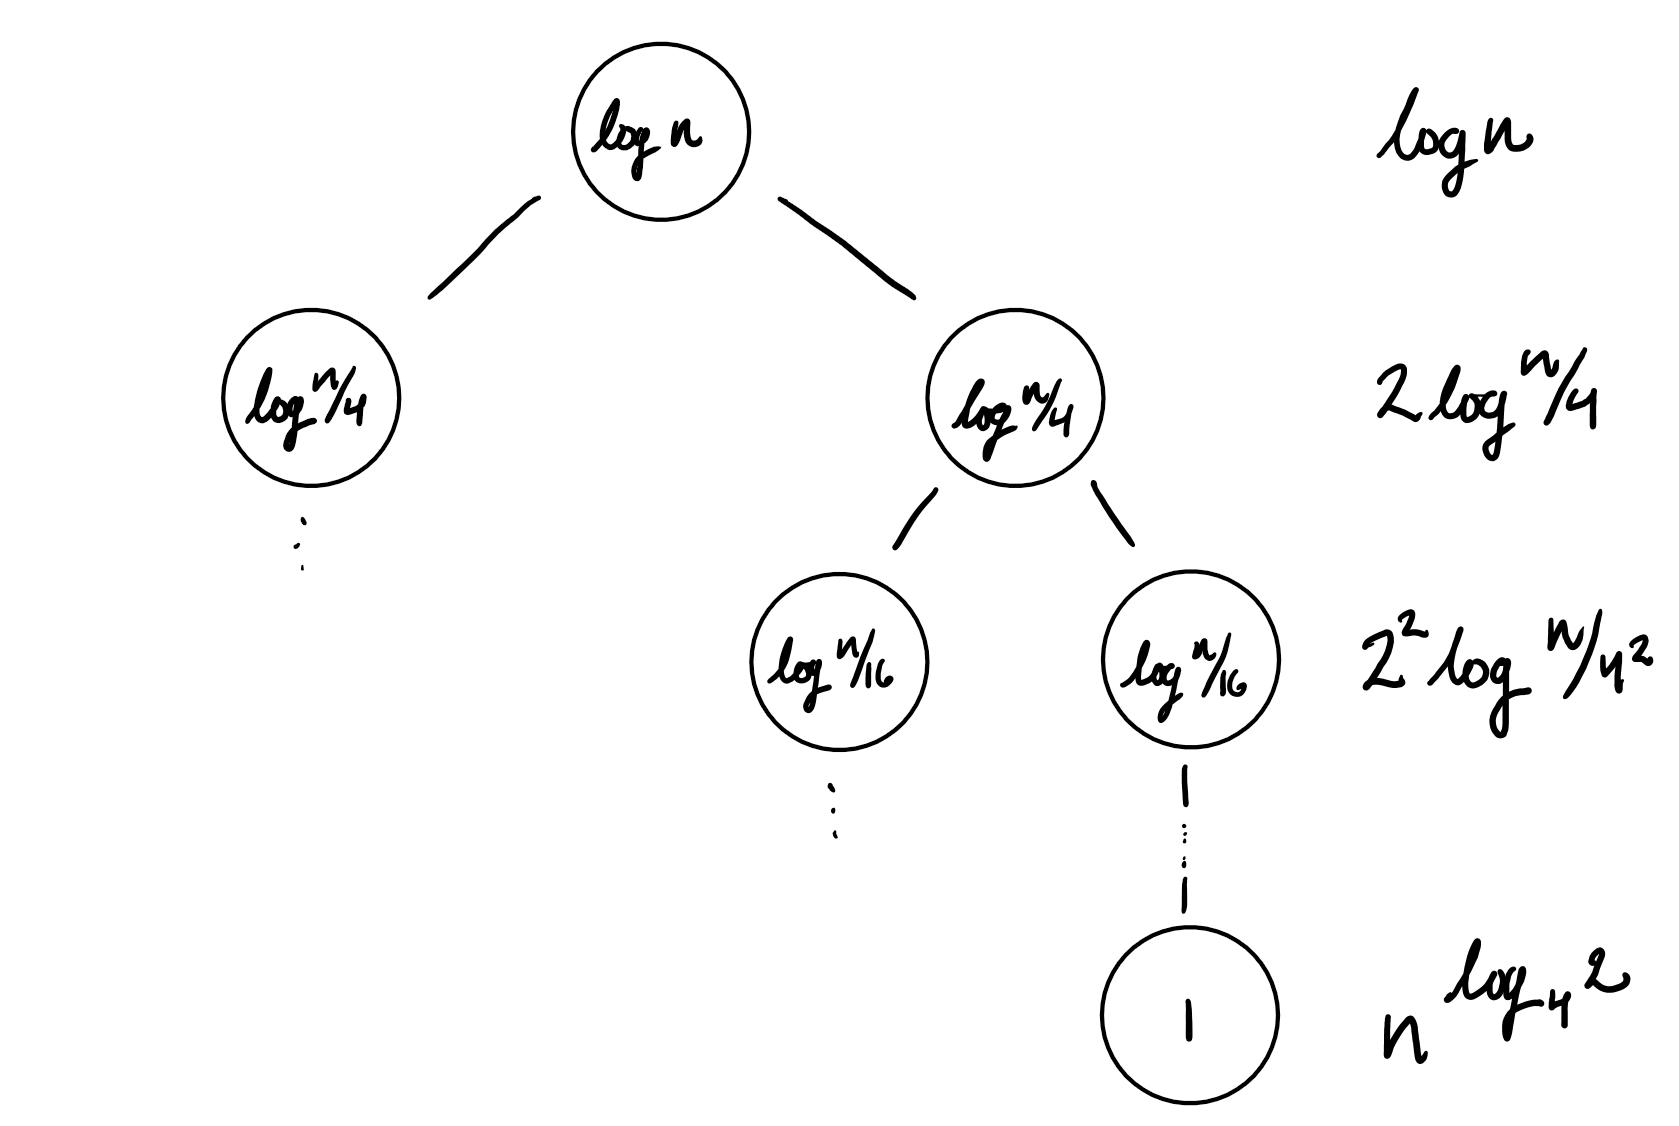
\includegraphics[scale=0.4]{Images/i.PNG}
    \end{center}
    From the recursion tree, $ T(n) = \log(n) + 2 \log (n/4) + 2^2 \log (n/4^2)
        + \ldots + n^{\log_4 2}$.  Looking at this sum shows the tree is
        leaf-heavy, that is, the leaves contribute more to the work. As a
        result, $ T(n) \in O(n^{\log_4 2}) $.
    \smallbreak
    Using the Master Theorem, $ a = 2 $, and $ b = 4 $. Checking the condition
        for Case I. In order for Case I to apply, $ \log n \in O(n^{\log_4 2 -
        \varepsilon} $ for some $ \varepsilon > 0 $. It is known from proof via
        textbook/recitation that $ (\log n)^a \in O(n^b) \forall a,b > 0 $.
        Therefore, if $ \varepsilon < 0.5 $ then $ \log n \in O(n^{\log_4 2 -
        \varepsilon}) $ and thus Case I applies. From this, $ T(n) \in
        \Theta(n^{\log_4 2}) $.
  \item $ T(n) = 17 T(n/3) + \Theta(n!) $
    \begin{center}
        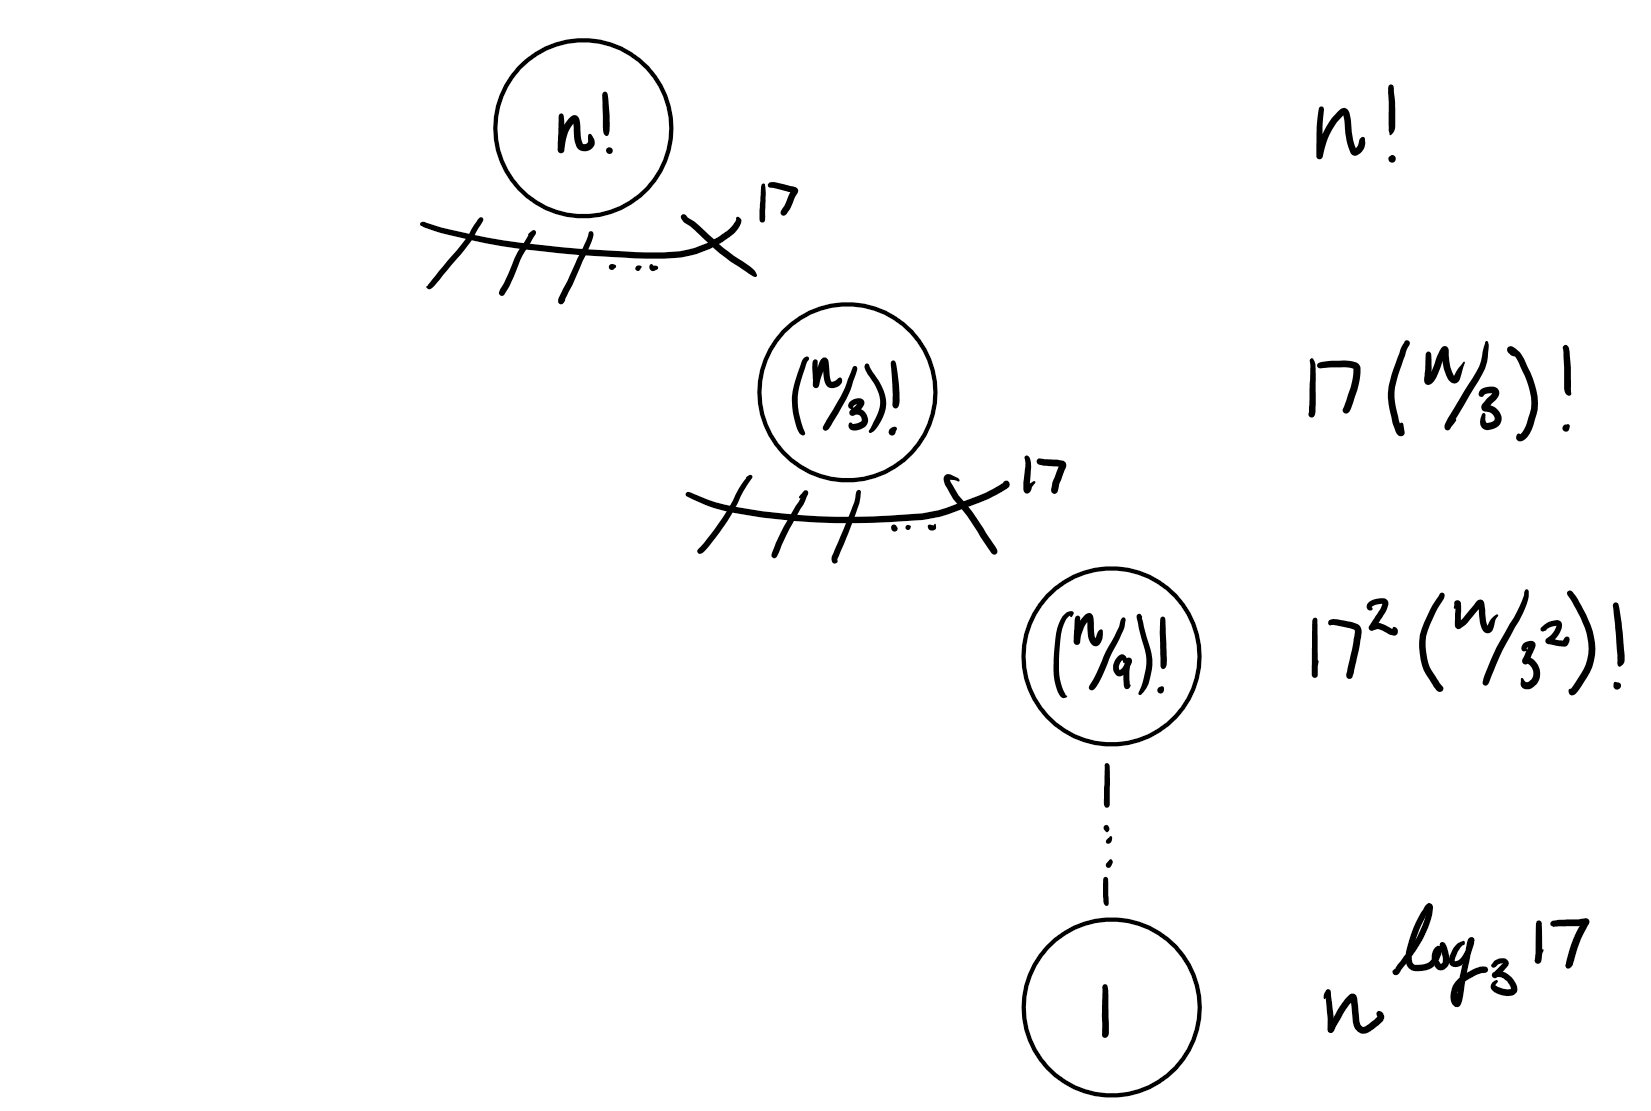
\includegraphics[scale=0.4]{Images/ii.PNG}
    \end{center}
    From the recursion tree, $ T(n) = n! + 17 (n/3)! + 17^2 (n/3^2)! + \ldots +
        n^{\log_3 17} $. Looking at this sum shows the tree is root-heavy, that
        is, the root contributes most to the work. As a result,
    $ T(n) \in O(n!) $.
    \smallbreak
    Using the Master Theorem, $ a = 17 $ and $ b = 3 $. Checking the condition
        for Case III. In order for Case III to apply, $ n! \in \Omega(n^{\log_3
        17 + \varepsilon} $ for some $ \varepsilon > 0 $. It is clear that a
        factorial is asymptotically greater than a polynomial. Therefore, $ n!
        \in \Omega(n^{\log_3 17 + \varepsilon} $ when $ \varepsilon = 1 $, for
        example. Furthermore, Case III requires $ 17 (n/3)! < c n! $ for some $
        0 < c < 1 $. Taking the limit of the ratio gives:
    $$ \lim_{n \to \infty} \frac{17(n/3)!}{c n!} $$
    The constants can be ignored
    $$ \lim_{n \to \infty} \frac{(n/3)!}{n!} $$
    Cancelling like terms
    $$ \lim_{n \to \infty} \frac{1}{n (n-1) \ldots (n/3 + 1)} = 0 $$
    Therefore, for any nonzero $ c $, $ 17 (n/3)! < c n! $ and Case III applies.
        From this, $ T(n) \in
    \Theta(n!) $
  \item $ T(n) = 25 T(n/5) + n^2 + 2n + \log n $
    \begin{center}
        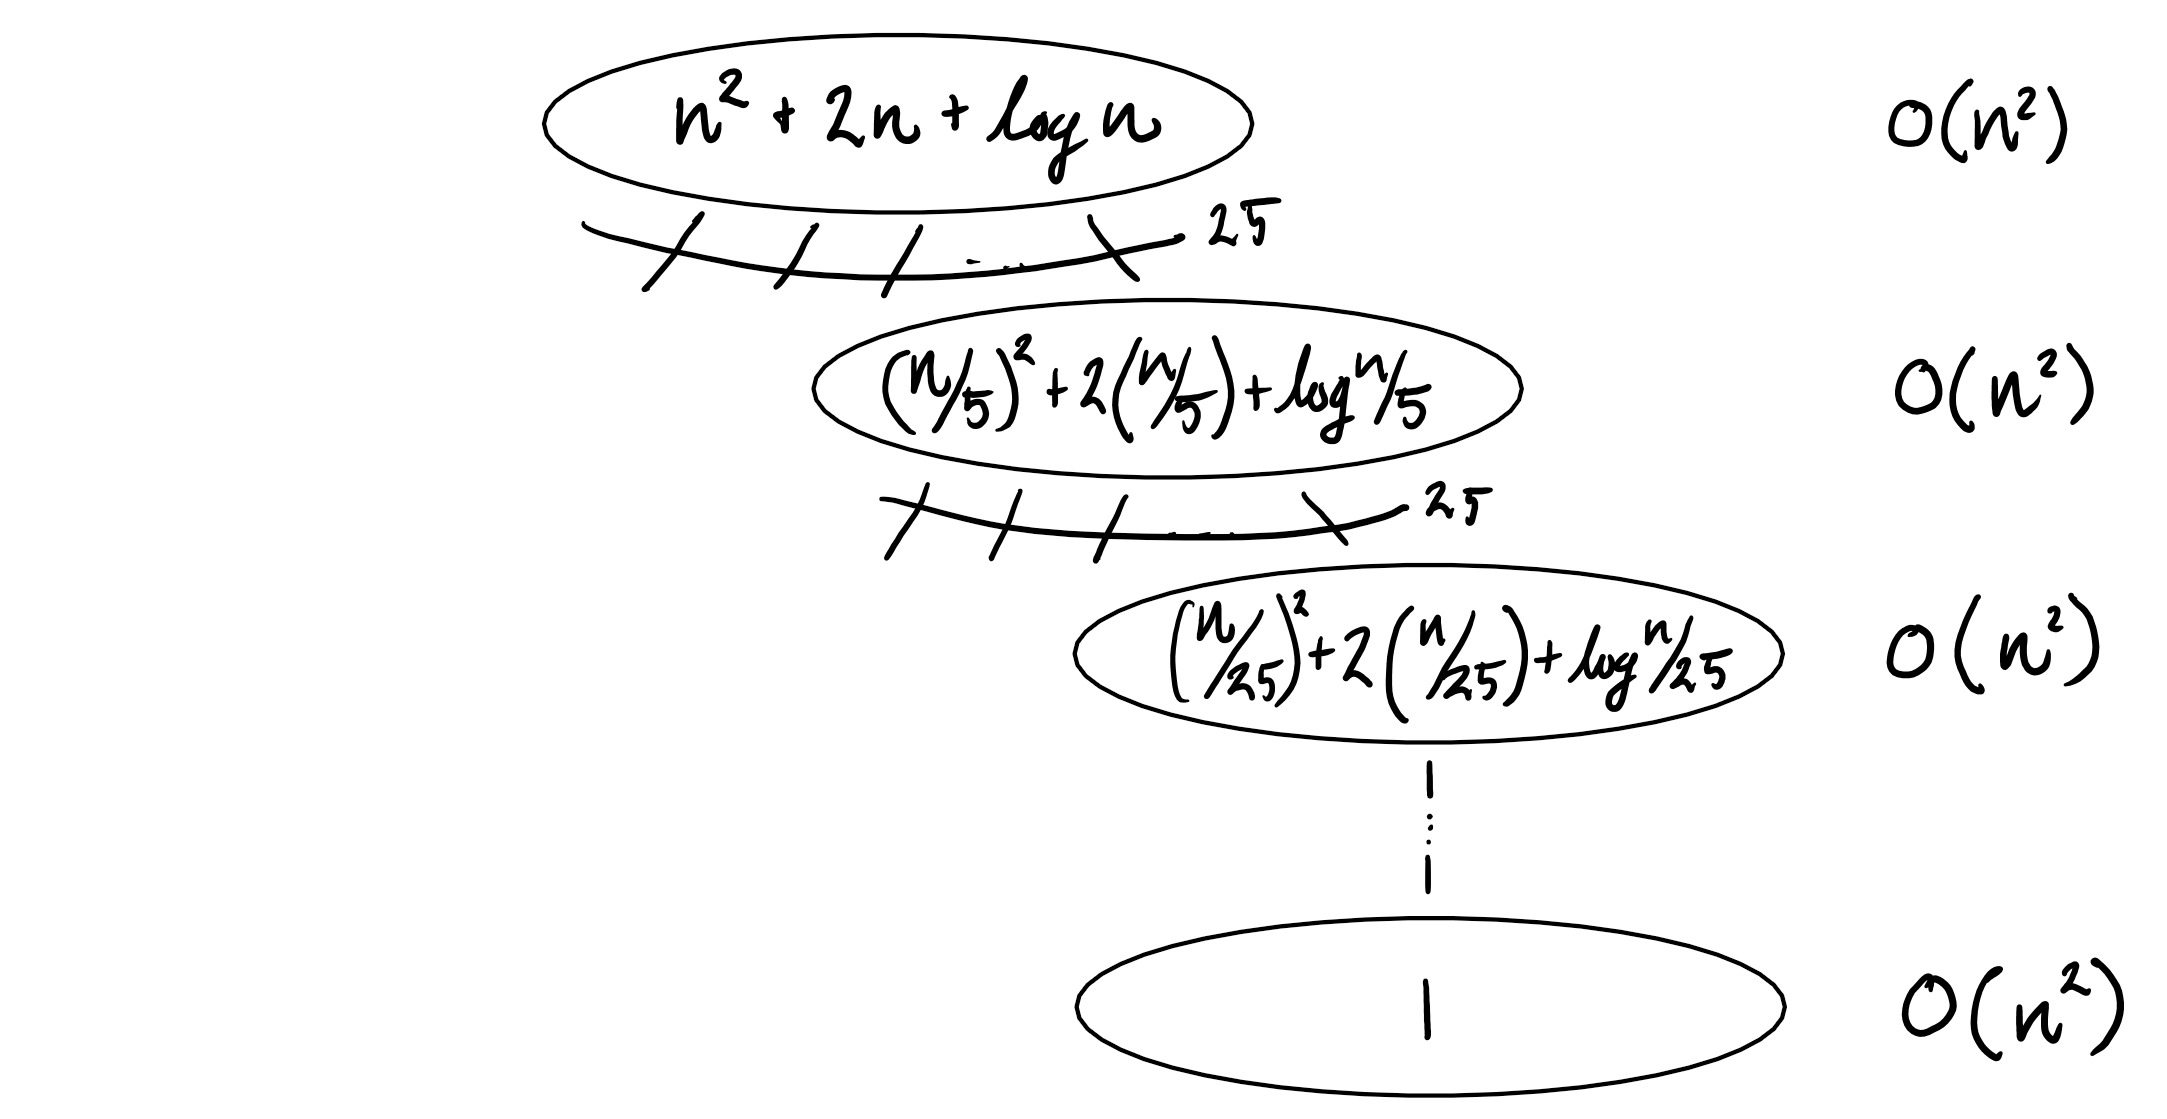
\includegraphics[scale=0.36]{Images/iii.PNG}
    \end{center}
    From the recursion tree, $ T(n) = O(n^2) + O(n^2) + \ldots + O(n^2) $.
        Looking at this sum shows the tree is even per level. Therefore, the
        total work is the work per level times the number of levels.  Since
        there are $ \log_5 n $ levels, $ T(n) \in O(n^2 \log n) $.
    \smallbreak
    Using the Master Theorem, $ a = 25 $ and $ b = 5 $. Checking the condition
        for Case II. In order for Case II to apply, $ n^2 \in \Theta(n^{\log_5
        25} \log^k n $ for some $ k \geq 0 $. It is easy to see that $ n^2 \in
        \Theta(n^2) $ therefore, $ n^2 \in \Theta(n^{\log_5 25} \log^k n $ for $
        k = 0 $. Thus Case II applies. From this, $ T(n) \in \Theta(n^2 \log n)
        $
  \item $ T(n) = T(\sqrt{n}) + O(1) $
      \begin{center}
          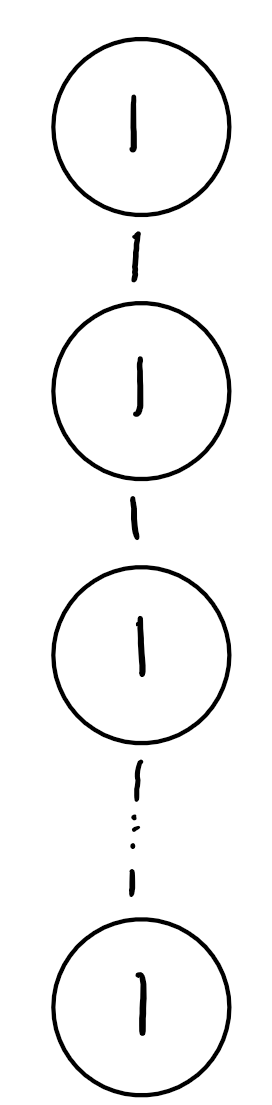
\includegraphics[scale=0.4]{Images/iv.PNG}
      \end{center}
      From the recursion tree, $ T(n) = 1 + 1 + \ldots + 1 $. Therefore the work
        is constant per level and only depends on the length of the chain. Given
        that at each level $ k $, $ n = n^{1/2^k} $, setting this equal to a
        termination point will allow solving for $ k $. Setting termination at $
        2 $, since $ 1 $ is never reached, yields $ n^{1/2^k} = 2 $. Solving for
        $ k $ results in $ k = \log \log n $.  Therefore, $T(n) \in O(\log \log
        n)$.
\end{enumerate}
\end{problemparts}

\newpage
\problem  % Problem 3

\begin{problemparts}
\problempart \textbf{Description} Iterate over each row and apply binary search.
    If the element is found within the row, terminate and return the index. If
    the element is not found, move to the next row until the are no remaining
    rows. If there are no more remaining rows, the element is not in the 2D
    array, return None.
    \smallbreak
    \textbf{Correctness} If the element is in the 2D array, it must be within at
    least one row. If it is in a row, the iteration will encounter that row and
    binary search will return its index. If the element is not in the 2D array,
    it will not be in a row and thus when the iteration completes through all
    rows without breaking early, it is certain the element is not in the array
    and will return None.
    \smallbreak
    \textbf{Running Time} Since each row has $ m $ elements, binary search on
    any of them will execute in $ O(\log m) $ time. Since there are $ n $ rows,
    the total complexity is $ O(n \log m) $.
\problempart If $ v > s $, then we can eliminate the first column of the 2D
    array. If $ v < s $, then we can eliminate the last row of the 2D array. If
    $ v \neq s $, then either a column or row will be eliminated. This means
    that either $ n $ or $ m $ elements will be removed. Therefore, at least $
    \min (n, m) $ elements are removed.
\problempart \textbf{Description} Initialize $ (x, y) $ to $ (0, n) $. Let $ s $
    be the element located at $ (x, y) $. If $ v > s $ (and $ x < m - 1 $),
    recurse after incrementing $ x $, thereby removing the first column of the
    array. Else if $ v < s $ (and $ y > 0 $), recurse after decrementing $ y $,
    thereby removing the last row of the array. Else if $ v = s $, the element
    has been found, return $ (x, y) $.  Else, return None as the bounds of the
    array have been met.
    \smallbreak
    \textbf{Correctness} Since each column and row are sorted increasing down
    and to the right, if the lowest, leftmost cell, $ s $, of a 2D-subarray is
    less than $ v $, and since all the elements above $ s $ are less than $ s $,
    then these elements can be removed as they are less than $ v $. Furthermore,
    if the $ s $ is greater than $ v $, and since all the elements to the right
    of $ s $ are greater than $ s $, then these elements can be removed as they
    are greater than $ v $. Given that $ v $ cannot be removed from the array by
    mistake, it must appear in the lower, leftmost cell of a 2D-subarray at some
    point if it is present in the array. Otherwise, the bounds of the array are
    met and None is returned.
    \smallbreak
    \textbf{Running Time} A recurrence can be constructed for this algorithm as
    follows $ T(m + n) = T(m + n - 1) + O(1) $ where $ n $ and $ m $ represent
    the number of rows and columns respectively. Each recurrence removes either
    one row or one column. At each step, the only operations are done in
    constant time. This recurrence is simply a chain of length $ m + n $ with
    each node of constant time. Therefore, $ T(n) \in O(n + m) $.
\problempart Submit your implementation to {\small\url{alg.mit.edu}}.
\end{problemparts}

\end{problems}

\end{document}


